\let\negmedspace\undefined
\let\negthickspace\undefined
\documentclass[journal]{IEEEtran}
\usepackage[a5paper, margin=10mm, onecolumn]{geometry}
%\usepackage{lmodern} % Ensure lmodern is loaded for pdflatex
\usepackage{tfrupee} % Include tfrupee package

\setlength{\headheight}{1cm} % Set the height of the header box
\setlength{\headsep}{0mm}     % Set the distance between the header box and the top of the text

\usepackage{gvv-book}
\usepackage{gvv}
\usepackage{cite}
\usepackage{amsmath,amssymb,amsfonts,amsthm}
\usepackage{algorithmic}
\usepackage{graphicx}
\usepackage{textcomp}
\usepackage{xcolor}
\usepackage{txfonts}
\usepackage{listings}
\usepackage{enumitem}
\usepackage{mathtools}
\usepackage{gensymb}
\usepackage{comment}
\usepackage[breaklinks=true]{hyperref}
\usepackage{tkz-euclide}
\usepackage{listings}                                     
\def\inputGnumericTable{}                                 
\usepackage[utf8]{inputenc}                                
\usepackage{color}                                            
\usepackage{array}                                            
\usepackage{longtable}                                       
\usepackage{calc}                                             
\usepackage{multirow}                                         
\usepackage{hhline}                                           
\usepackage{ifthen}                                           
\usepackage{lscape}
\renewcommand{\thefigure}{\theenumi}
\renewcommand{\thetable}{\theenumi}
\setlength{\intextsep}{10pt} % Space between text and floats

\numberwithin{equation}{enumi}
\numberwithin{figure}{enumi}
\renewcommand{\thetable}{\theenumi}

% Marks the beginning of the document
\begin{document}
\bibliographystyle{IEEEtran}

\title{Question-16.4.4.1}
\author{EE24BTECH11048-NITHIN.K} 
%\maketitle
%\newpage
%\bigskip
{\let\newpage\relax\maketitle}
\textbf{Question:}\\
Out of 100 students, two sections of 40 and 60 are formed. If you and your friend are among the 100 students, what is the probability that you both enter the different section.
\textbf{Solution:}\\
We model this problem using Bernoulli random variables,\\
Let X be a Bernoulli random variable representing the section assignment of a student:\\
\begin{align*}
	\text{X = 1 if a student is assigned to Section 1 (with probability p = 0.4)}
\end{align*}
\begin{align*}
	\text{X = 0 if a student is assigned to Section 2 (with probability 1 - p = 0.6)}
\end{align*}
Similarly, define another Bernoulli random variable Y for your friend with the same probabilities.\\
\textbf{Consider the Joint Probabilities:}\\
Since the assignments are independent, the joint probabilities are:\\
\textbf{Different Sections:}\\
X = 1, Y = 0 (You in Section 1, friend in Section 2):
\begin{align}
	P\brak{X = 1, Y = 0} = P\brak{X = 1}P\brak{Y = 0} = 0.4 \times 0.6 = 0.24
\end{align}
\begin{align}
        P\brak{X = 0, Y = 1} = P\brak{X = 0}P\brak{Y = 1} = 0.6 \times 0.4 = 0.24
\end{align}
\textbf{Compute Probabilities:}\\
Probability that both enter different sections:\\
\begin{align}
	P\brak{X \neq Y} = P\brak{X = 1, Y = 0} + P\brak{X = 0, Y = 1} = 0.24 + 0.24 = 0.48
\end{align}
\textbf{PMF:}
The PMF of a Bernoulli random variable X is given by:
\begin{align}
	P\brak{X = x} = p^x\brak{1 - p}^{1 - x}, x \in \cbrak{0,1}
\end{align}
substituting p = 0.4,\\
\begin{align}
 P\brak{X = 1} = 0.4, P\brak{X = 0} = 0.6
\end{align}
\begin{align}
	P\brak{X = x} = \begin{cases}
		0.4, & x = 1 \\
		0.6, & x = 0 \\
		0, & \text{otherwise}
	\end{cases}
\end{align}
\textbf{CDF:}\\
The CDF of a discrete random variable is defined as:\\
\begin{align}
	F\brak{x} = P\brak{X \leq x}
\end{align}
\begin{align}
        F\brak{x} = \begin{cases}
                0, & x < 0 \\
                0.6, & 0 \leq x < 1  \\
                1, & x \geq 1
        \end{cases}
\end{align}
Since Y (your friend's section assignment) follows the same Bernoulli distribution as X, its probability mass function (PMF) and cumulative distribution function (CDF) are identical to those of X.\\
\begin{figure}[H]
    \centering
    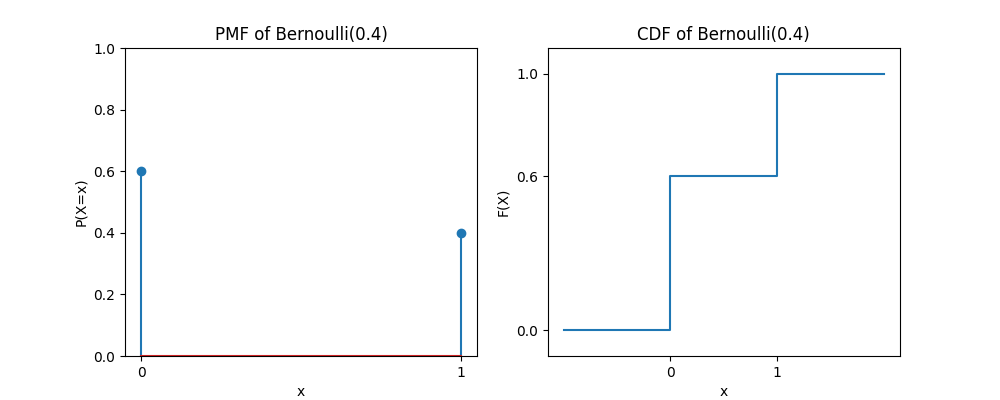
\includegraphics[width=\textwidth]{figs/fig.png}
\end{figure}

\end{document}
